\label{chap:NoGANs}

Der Lernfortschritt von Klassifikatoren besteht darin, besser in der Aussage zu werden, ob eine Vorhersage $y$ auf einen gegebenen Eingang $x$ zutrifft. Das bezeichnet man auch als \emph{diskriminative Modellierung}. Um das zu erlenen, benötigt der Klassifikator annotierte Trainingsdaten. Das bedeutet, dass jedes Trainingsbeispiel $x$ eine erwartete Vorhersage $y$ besitzt. Man bezeichnet das auch als \emph{überwachtes Lernen}. \cite{generative-modellierung}

Neben der diskriminativen Modellierung ist auch eine \emph{generative Modellierung} möglich. Generative \acp{KNN} lernen, neue Daten zu erzeugen, die der Verteilung der Trainingsdaten ähneln. Dazu erlernen sie die statistische Verteilung der Trainingsdaten. Generative Netze zur Bilderzeugung können demnach Bilder generieren, die vergleichbar mit den Trainingsbildern sind. Beispielsweise wenn ein generarives Modell darauf trainiert ist, Katzenbilder zu erzeugen. Die Trainingsbilder sind nicht annotiert, wodurch generative Netze in der Regel in das \emph{unüberwachte Lernen} einzuordnen sind. \cite{generative-modellierung}

\subsection{Mathematischer Hintergrund}
Generative Netze zur Bilderzeugung sollen beurteilen können, wie wahrscheinlich es ist, dass ein gegebenes Bild aus der Verteilung der Trainingsdaten stammt. Wenn $x$ für jedes mögliche existierende Bild steht, so bilden generative Netze folgende Wahrscheinlichkeitsverteilung ab: \cite{generative-modellierung}
\begin{equation}
   \hat{p}(x)
\end{equation}
Für ein gegebenes Bild $x$ gibt $\hat{p}(x)$ einen Schätzwert dafür an, wie wahrscheinlich es ist, dass das Bild aus den Trainingsdaten stammt. Diese Wahrscheinlichkeitsverteilung wird durch das Netz erlernt. Das Training des generativen Netzes optimiert, dass die geschätzte Verteilung der Daten $\hat{p}(x)$ möglichst ähnlich zu der tatsächlichen Verteilung der Trainingsdaten $p(x)$ ist. Ein beispielhafter Vergleich ist in Abbildung \ref{fig:generativeNetsPx} dargestellt. Es ist erkennbar, dass sich die geschätzte und die tatsächliche Verteilung ähnlich sehen, jedoch nicht identisch sind. Die Abweichung zwischen diesen Verteilungen stellt dabei die Kosten dar. Die schwarzen Punkte kennzeichnen Trainingsdaten. Sie sollen die Verteilung $p(x)$ abbilden. Weniger diversifizierte Trainingsdaten würden sich beispielsweise nur in einem Teilbereich von $p(x)$ befinden. Dadurch könnte das Modell $p(x)$ weniger gut approximieren. \cite{generative-modellierung} \cite{openAiGenerativeNets}

\begin{figure}[H]
   \centering
   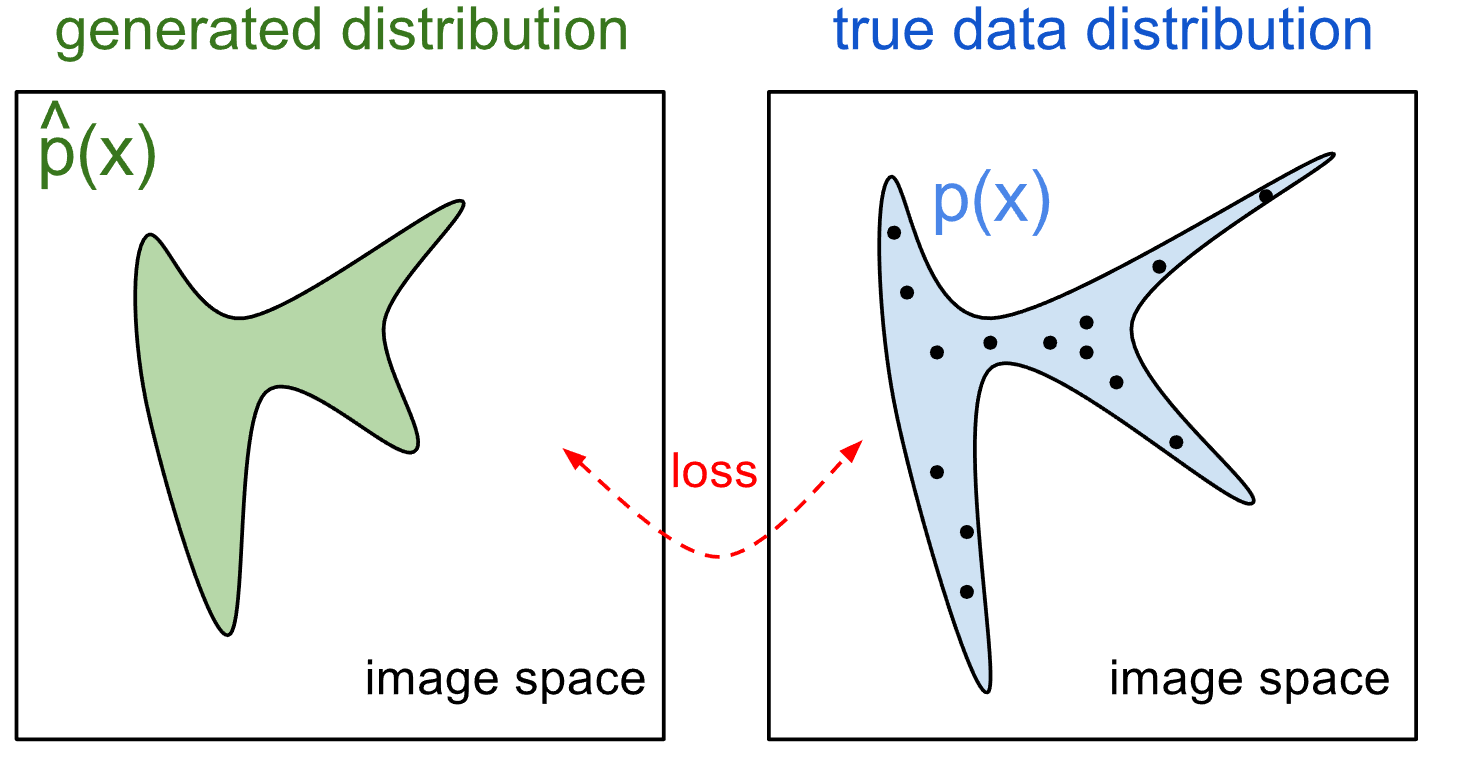
\includegraphics[width=0.5\textwidth]{images/Generative Networks/p(x) Distribution.png}
   \caption{Beispielhafter Vergleich von $\hat{p}(x)$ und $p(x)$ \cite{openAiGenerativeNets}}
   \label{fig:generativeNetsPx}
\end{figure}

Bei der Bildgenerierung versucht das Netz den Wahrscheinlichkeitswert für $\hat{p}(x)$ zu maximieren. Es erlernt durch $\hat{p}(x)$, wie die Verteilung der Trainingsdaten aussieht und versucht anschließend ausschließlich Bilder zu generieren, die dieser Verteilung folgen. Bezogen auf Abbildung \ref{fig:generativeNetsPx} befinden sich alle generierten Bilder des trainierten Netzes im grün markierten Bereich. \cite{generative-modellierung} \cite{openAiGenerativeNets}

Es existieren verschiedene Arten generativer Netze. Die Taxonomie, also die Einteilung verschiedener Netze in bestimmte Kategorien, stellt Abbildung \ref{fig:generativeModelsTaxonomy} dar. Einerseits existieren Architekturen, die die Wahrscheinlichkeitsverteilung $\hat{p}(x)$ explizit berechnen oder approximieren. Andere berechnen die Funktion nicht, verwenden sie jedoch implizit. Die Abbildung unterscheidet dahingehend zwischen den Kategorien \emph{Explizite Wahrscheinlichkeitsdichte} und \emph{Implizite Wahrscheinlichkeitsdichte}. Auf der untersten Ebene der Taxonomie befinden sich konkrete Architekturen generativer Netze. Dabei sind nur diejenigen aufgeführt, die diese Studienarbeit in betracht zieht. Die Auswahl basiert auf verschiedenen Veröffentlichungen, die Architekturen für generative Netze vergleichen \cite{generative-models-comparison} \cite{generativeModelsSurvey}. Abbildung \ref{fig:generativeModelsTaxonomy} deutet jedoch an, dass darüber hinaus weitere Arten existieren. \cite{generativeModelsBook}

\usetikzlibrary{shadows.blur}
\begin{figure}[h]
   \centering
   \begin{forest}
      forked edges,
      for tree={font=\sffamily, rounded corners, top color=white, bottom color=white, edge+={darkgray, line width=1pt}, draw=darkgray, align=center, anchor=children},
      before packing={where n children=3{calign child=2, calign=child edge}{}},
      before typesetting nodes={where content={}{coordinate}{}},
      where level<=1{line width=2pt}{line width=1pt},
      [Generative Modelle, blur shadow, line width=1pt
        [Explizite Wahrscheinlichkeitsdichte, line width=1pt
          [Berechenbar, line width=0mm
            [\acs{PixelRNN}, line width=0mm, fill=encoder]
            [..., line width=0mm, fill=encoder]
          ]
          [Approximiert, line width=0mm
            [\acs{VAE}, line width=0mm, fill=encoder]
            [..., line width=0pt, fill=encoder]
          ]
        ]
        [Implizite Wahrscheinlichkeitsdichte, line width=1pt
          [Direkt, line width=0mm
            [\acs{GAN}, line width=0mm, fill=encoder]
          ]
          [Markov-Kette, line width=0mm
            [..., line width=0pt, fill=encoder]
          ]
        ]
      ]
    \end{forest}
   \caption{Taxonomie generativer Modelle \emph{angelehnt an \cite{generativeModelsBook}}}
   \label{fig:generativeModelsTaxonomy}
\end{figure}

%\begin{figure}[h]
%   \centering
%   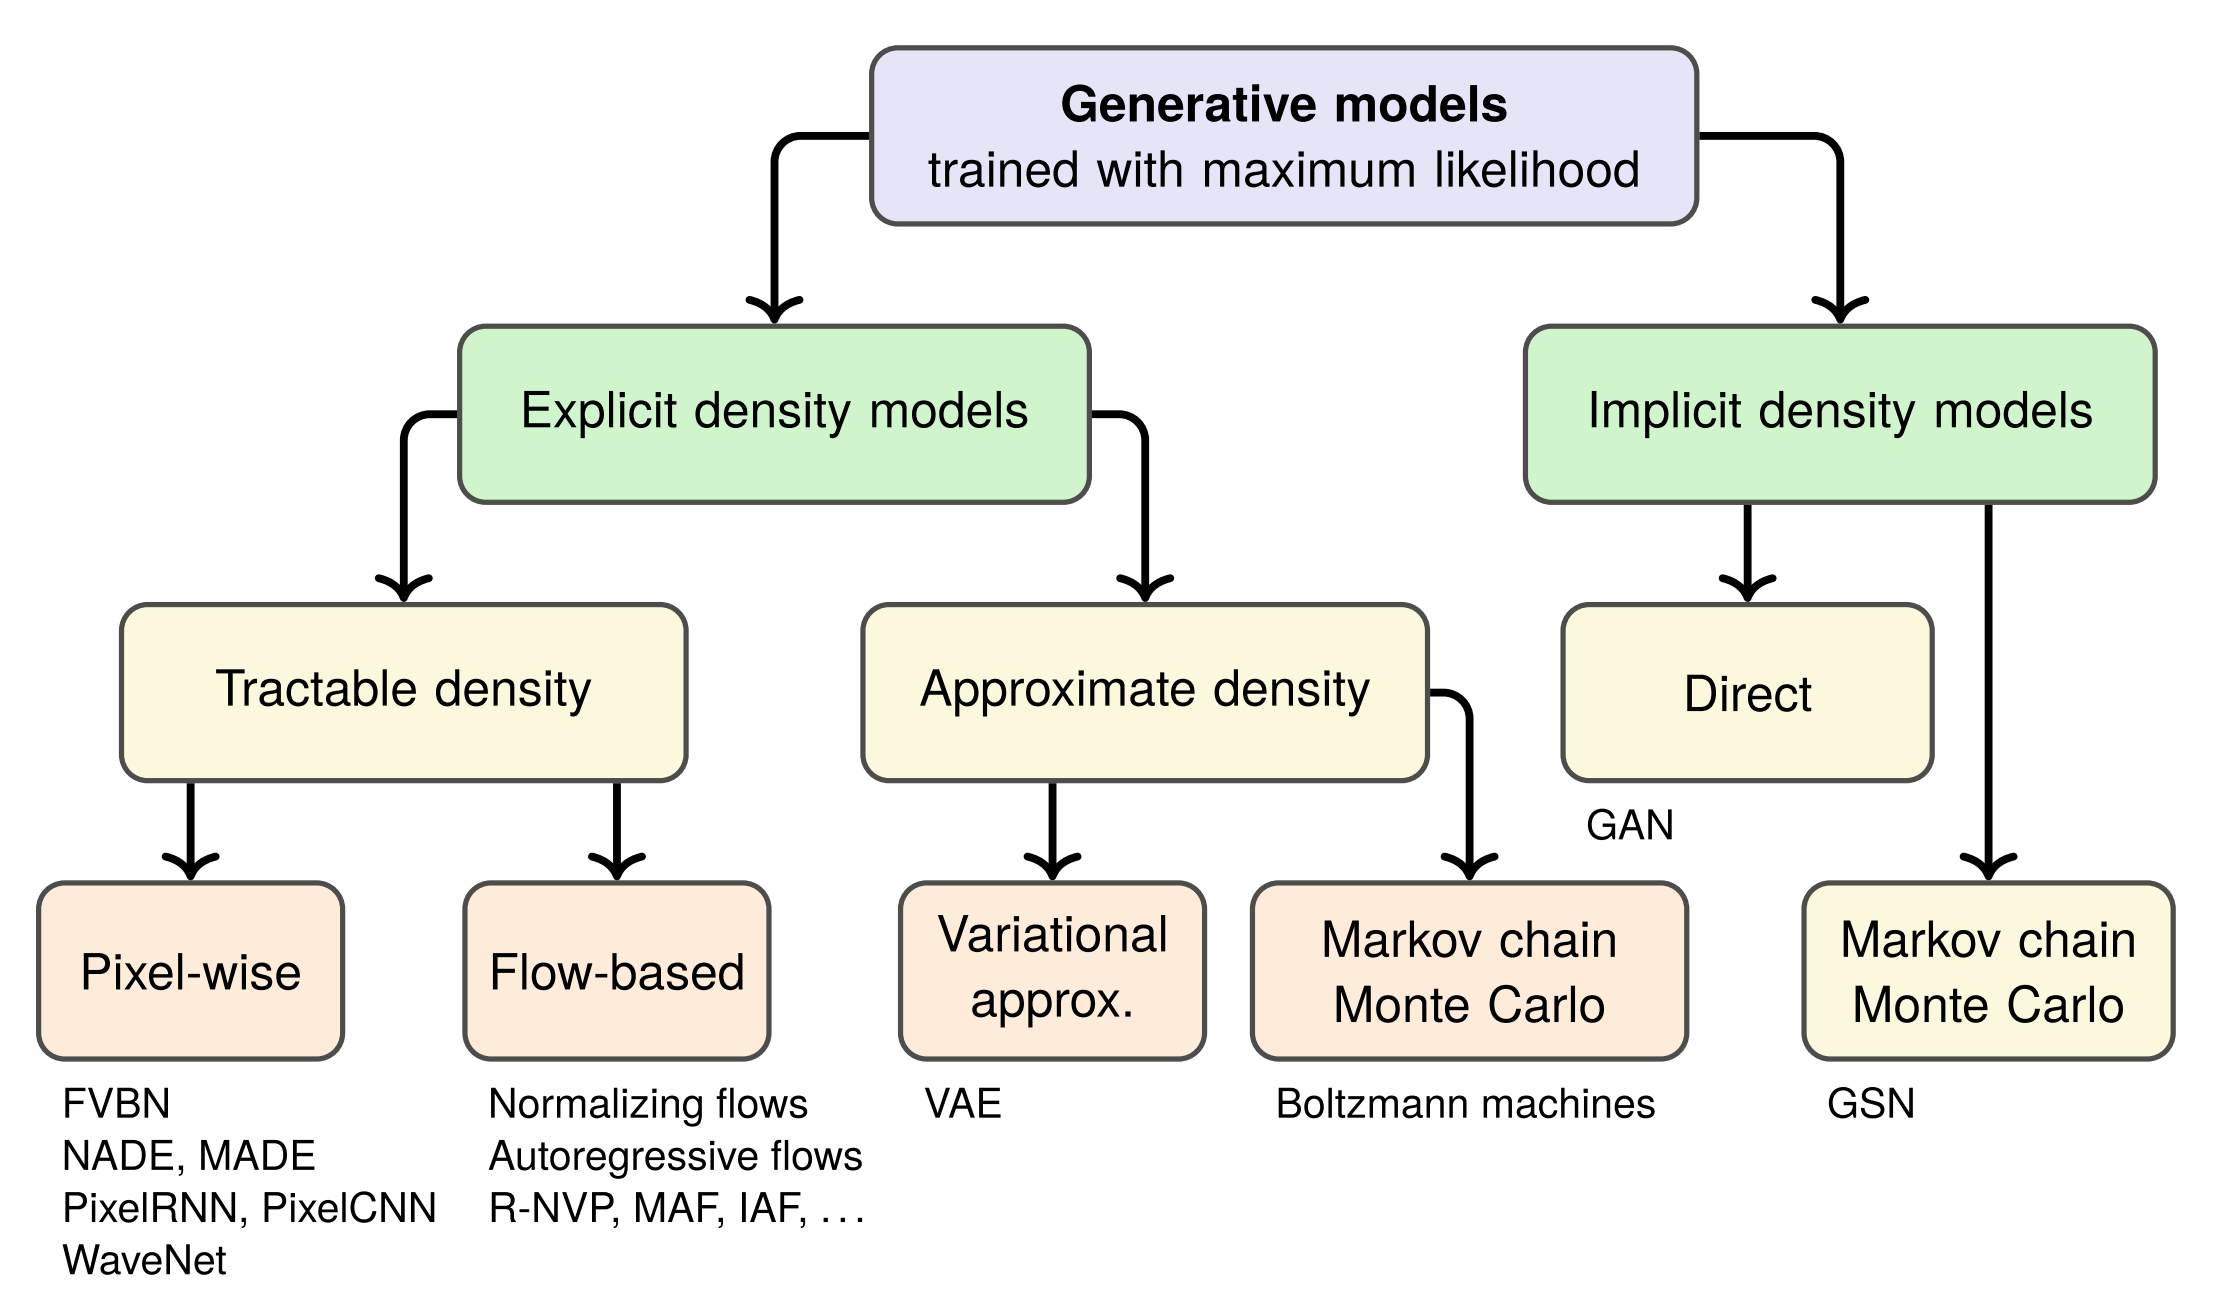
\includegraphics[width=0.8\textwidth]{images/Generative Networks/Taxonomy of Generative Models.png}
%   \caption{Taxonomie generativer Modelle \cite{generativeModelsBook}}
%   \label{fig:generativeModelsTaxonomy}
%\end{figure}

Dieses Kapitel soll auf die gezeigten Architekturen eingehen, um ein Verständnis für die Funktionsweise generativer Netze zu schaffen. Darauf basierend trifft Kapitel \ref{chap:3-architektur} eine Auswahl für die Architektur, die für diese Studienarbeit verwendet wird.

\subsection{Pixel Recurrent Neural Networks}
Die Architektur der \acp{PixelRNN} stammt aus dem Jahre 2016. Diese Netze stützen sich explizit auf die Maximierung der Maximum-Likelihood-Schätzung von $\hat{p}(x)$ für jeden Pixel. Sie sind in der genannten Taxonomie den Modellen zuzuordnen, die den tatsächlichen Schätzwert von $p(x)$ berechnen können. \cite{pixelRNN}

Im folgenden soll geklärt werden, wie ein \ac{PixelRNN} den optimalen Wert für jeden Pixel eines generierten Bildes bestimmt. Ein betrachtetes Bild $x$ der Auflösung $n \times n$ kann in seine einzelnen Pixel $(x_{1}, x_{2}, ..., x_{n^2})$ aufgeteilt werden. Gleichung \ref{eq-max-likelihood} gibt an, wie die Wahrscheinlichkeit eines jeden Pixels in die gesamte Verteilung $\hat{p}(x)$ einfließt. \cite{pixelRNN}
\begin{equation}
   \label{eq-max-likelihood}
   \hat{p}(x) = \hat{p}(x_{1}, x_{2}, ..., x_{n^2}) = \prod_{i=1}^{n^2}\hat{p}(x_{i}|x_{1},...,x_{i-1})
\end{equation}
Jeder Pixel $x_{i}$ besitzt eine eigene Wahrscheinlichkeitsverteilung $\hat{p}(x_{i}|x_{1},...,x_{i-1})$. Sie ist abhängig von allen anderen Pixeln $x_{1},...,x_{i-1}$ des Bildes. Den optimalen Wert jedes Pixels kann das \ac{PixelRNN} demnach nur dann berechnen, wenn die Werte aller anderen Pixel bekannt sind. Das Produkt aller Wahrscheinlichkeitswerte der einzelnen Pixel ergibt $\hat{p}(x)$. Soll $\hat{p}(x)$ maximiert werden, so müssen die Terme $\hat{p}(x_{i}|x_{1},...,x_{i-1})$ möglichst hohe Werte liefern. Daraus ergibt sich dann unter gegebenem Kontext für jeden Pixel eine Maximum-Likelihood-Schätzung. Also der Pixelwert, für den $\hat{p}(x)$ möglichst weit gegen \emph{eins} strebt. \cite{pixelRNN}

Die Idee von PixelRNNs ist, dass die Generierung in einer Ecke des Bildes startet. Das Bild wird zunächst auf einen Pixel reduziert, der im folgenden $x_{1}$ genannt wird. Für diesen Pixel generiert das \ac{PixelRNN} einen Wert. Anschließend wird $x_{1}$ gemeinsam mit einem benachbarten Pixel $x_{2}$ betrachtet. Die Wahrscheinlichkeitsverteilung für $x_{2}$ ergibt sich dadurch zu $\hat{p}(x_{2}|x_{1})$. Der Wert für $x_2$ ist somit nur von $x_1$ abhängig. Da $x_{1}$ bekannt ist, kann das \ac{PixelRNN} einen optimalen Wert für $x_{2}$ bestimmen. Die Wahrscheinlichkeitsverteilung von $x_{3}$ ergibt sich zu $\hat{p}(x_{3}|x_{1}, x_{2})$, die von $x_{4}$ zu $\hat{p}(x_{4}|x_{1}, x_{2}, x_{3})$. Das \ac{PixelRNN} generiert das Bild sukzessive, wobei der momentane Pixelwert für $x_{i}$ von allen bisher generierten Pixeln abhängt. Dieses vorgehen ist in Abbildung \ref{fig:pixelRNN} dargestellt. Der Wert des rot markierten Pixels hängt von allen blau markierten Pixel ab. Ist für diesen ein Wert bestimmt, wird der rechtsseitig benachbarte Pixel als neues $x_{i}$ gewählt.

\begin{figure}[h]
   \centering
   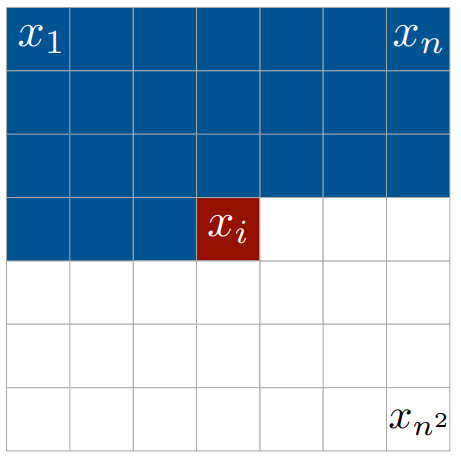
\includegraphics[width=0.25\textwidth]{images/Generative Networks/PixelRNN.png}
   \caption{Bestimmung von $\hat{p}(x)$ mit PixelRNNs \cite{pixelRNN}}
   \label{fig:pixelRNN}
\end{figure}

Um die beschriebene Abhängigkeit des momentan generierten Pixels zu allen bisher generierten Pixel umsetzen zu können, besitzen \acp{PixelRNN} eine Art \emph{Erinnerung}. Bisher wurden in dieser Arbeit nur sogenannte \emph{Feedforward} Netze behandelt, bei denen der Informationsfluss stets in eine Richtung erfolgt. Nämlich vom Eingang des Netzes zum Ausgang. Es existieren auch \emph{Recurrent Neural Networks}. Sie werden besonders zur Verarbeitung von natürlicher Sprache eingesetzt \emph(engl.: natural language processing).

%\begin{figure}[h]
   %\centering
   %\includegraphics[width=0.375\textwidth]{images/Generative Networks/%RNN.png}
%   \caption{Darstellung eines Recurrent Neural Networks \cite{ibmRNN}}
%   \label{fig:RNN}
%\end{figure}

In Recurrent Neural Networks spielen die \emph{Zustände} eines Netzes eine besondere Rolle. Ein Zustand wird durch die Eingangs- und Ausgangswerte aller Neuronen zu einem gegebenen Zeitpunkt beschrieben. In \acp{PixelRNN} ist der Zustand des Netzes für den Pixel $x_{2}$ abhängig von dem Zustand des Netzes für $x_{1}$. Um solche Beziehungen darstellen zu können, besitzt ein Recurrent Neural Network Neuronen, die den vorherigen Wert eines Neurons rekursiv auf seinen Eingang zurückführen. Somit wird der vorherige Zustand des neuronalen Netzes als zusätzlicher Eingang für die Berechnungen genutzt. \acp{PixelRNN} nutzen eine besondere Form der Recurrent Neural Networks. Sie arbeiten mit sogenannter \emph{Long Short-term Memory}. Dadurch soll das Problem behoben werden, dass in klassischen Recurrent Neural Networks weit in der Vergangenheit liegende Zustände nur noch einen geringen Einfluss auf den momentanen Zustand haben. \cite{generativeModelsSurvey}

Da die durch ein \ac{PixelRNN} umgesetzte Verteilung $\hat{p}(x)$ direkt erfassbar ist, wird ihnen nachgesagt, dass die Performanz solcher Netze gut evaluiert werden kann. Es gilt als vergleichsweise leicht, für solche Netze Metriken zur Messung der Performanz umzusetzen. Ein grundlegender Nachteil von \acp{PixelRNN} ist hingegen, dass sie die Bilder nur sequenziell generieren können. Es ist in dem beschriebenen Verfahren nicht möglich, mehrere Pixel parallel zu erzeugen, da der Wert eines Pixels von denen aller vorher generierten Pixel abhängig ist. Dies verlangsamt die Generierung, da keine Parallelisierung möglich ist. \cite{generativeModelsSurvey}

Es existieren auch sogenannte \emph{PixelCNNs}, bei denen sich die Berechnung stets nur auf bestimmte Bildbereiche konzentriert. Diese Bildbereiche kann das PixelCNN parallel zueinander berechnen. Die Parallelisierung ist jedoch nur während des Trainings des Netzwerks oder während der Evaluation von $\hat{p}(x)$ für gegebene Bilder möglich. Die Bildgenerierung erfolgt auch hier, analog zu \acp{PixelRNN}, vollständig sequenziell. \cite{pixelRNN}

\subsection{Autoencoder}

Das Ziel von Autoencodern ist, den Eingang des Netzes am Ausgang zu rekonstruieren. Dazu setzen sich diese Netze aus drei Bestandteilen zusammen: dem Kodierer, dem latenten Raum und dem Dekodierer. In Abbildung \ref{fig:Autoencoder} ist eine beispielhafte Autoencoderarchitektur dargestellt. \cite{autoencoder}
\begin{figure}[h]
   \centering
   \begin{tikzpicture}[scale=0.8, transform shape,
      neuron/.style={circle,draw,thick,minimum size=0.6cm}]
   
      % Encoder hidden layers
      \foreach \h [count=\i] in {1,...,8}
         \node[neuron, fill=encoder-x] (enc-first\i) at (0,\h-4) {$x_{\i}$};
   
      \foreach \h [count=\i] in {1,...,6}
         \node[neuron, fill=encoder] (enc-second\i) at (2,\h-3) {};
   
      \foreach \h [count=\i] in {1,...,4}
         \node[neuron, fill=encoder] (enc-third\i) at (4,\h-2) {};
   
      \foreach \h [count=\i] in {1,...,2}
         \node[neuron, fill=latent] (enc-fourth\i) at (6,\h-1) {$z_{\i}$};
   
      % Decoder hidden layers
      \foreach \h [count=\i] in {1,...,4}
         \node[neuron, fill=decoder] (dec-first\i) at (8,\h-2) {};
   
      \foreach \h [count=\i] in {1,...,6}
         \node[neuron, fill=decoder] (dec-second\i) at (10,\h-3) {};
   
      \foreach \h [count=\i] in {1,...,8}
         \node[neuron, fill=decoder-x] (dec-third\i) at (12,\h-4) {$\hat{x}_{\i}$};
   
      % Connections
      \foreach \i in {1,...,8}
         \foreach \h in {1,...,6}
            \draw[lightgray] (enc-first\i) -- (enc-second\h);
   
      \foreach \i in {1,...,6}
         \foreach \h in {1,...,4}
            \draw[lightgray] (enc-second\i) -- (enc-third\h);
   
      \foreach \i in {1,...,4}
         \foreach \h in {1,...,2}
            \draw[lightgray] (enc-third\i) -- (enc-fourth\h);
   
      \foreach \i in {1,...,2}
         \foreach \h in {1,...,4}
            \draw[lightgray] (enc-fourth\i) -- (dec-first\h);
   
      \foreach \i in {1,...,4}
         \foreach \h in {1,...,6}
            \draw[lightgray] (dec-first\i) -- (dec-second\h);
   
      \foreach \i in {1,...,6}
         \foreach \h in {1,...,8}
            \draw[lightgray] (dec-second\i) -- (dec-third\h);
   
      \node[above] at (0, -4.5) {Eingang};
      \node[above] at (6,-1.5) {latenter Raum};
      \node[above] at (12,-4.5) {Nachgebildeter Eingang};
      \node[above, rotate=0, text=encoder-x] at (3, 4) {\large \textbf{Kodierer}};
      \node[above right, rotate=0, text=decoder-x] at (7.5, 4) {\large \textbf{Dekodierer}};
   \end{tikzpicture}
   %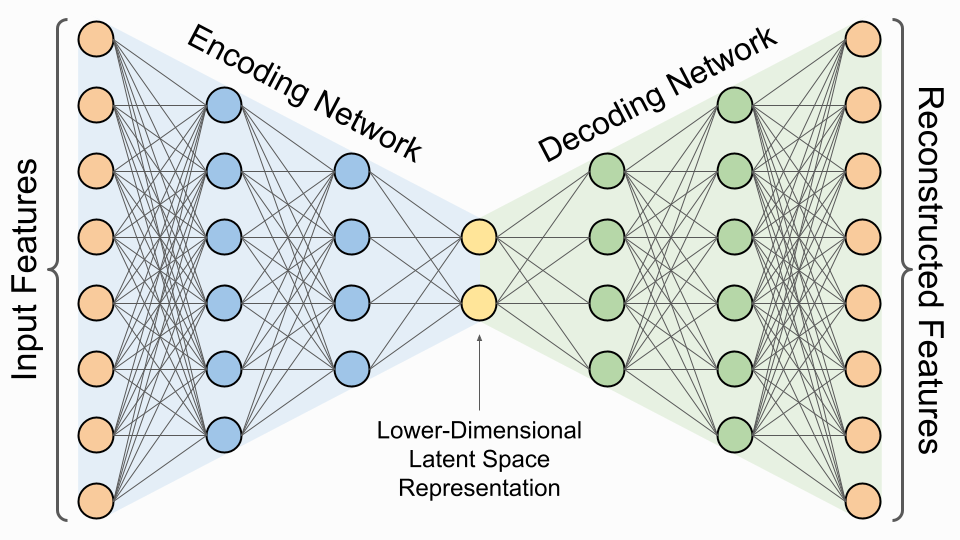
\includegraphics[width=0.65\textwidth]{images/Generative Networks/autoencoder_architecture.png}
   \caption{Architektur eines Autoencoders \emph{(angelehnt an \cite{autoencoder-img})}}
   \label{fig:Autoencoder}
\end{figure}

Der \textbf{Kodierer} besitzt die Aufgabe, Merkmale aus dem Eingang des Netzes zu extrahieren. Diese Merkmale sollen daraufhin mit einer begrenzten Anzahl an Parametern durch den latenten Raum repäsentiert werden. Somit besteht die Aufgabe des Kodierers darin, den Eingang auf seine für das Netz wesentlichen Eigenschaften zu reduzieren. Und zwar erfolgt die Komprimierung dabei so, dass die Informationen gerade so durch den latenten Raum dargestellt werden können. \cite{autoencoder}

Bei dem \textbf{latenten Raum} handelt es sich um eine einzelne Schicht von Parametern, oder in diesem Kontext: Neuronen. Je mehr Neuronen sich in dem latenten Raum befinden, desto mehr Informationen kann der Kodierer an den Dekorier übergeben. Ein Vektor $\vec{z}$ beschreibt beispielsweise die Merkmale, die sich in dem latenden Raum befinden. Der latente Raum sollte klein genug sein, damit der Kodierer in $\vec{z}$ nicht alle Merkmale des Eingangs speichern kann. So wird der Kodierer dazu gezwungen, vereinzeilte Merkmale zu extrahieren. \cite{autoencoder}

Der \textbf{Dekodierer} nutzt die Werte aus dem latenten Raum, um den Eingang nachzubilden. Diese Nachbildung stellt den Ausgang des Autoencoders dar. Die Kosten eines Autoencoders ergeben sich durch die Abweichung zwischen Ein- und Ausgang. \cite{autoencoder}

Da der Zweck von Autoencodern darin besteht, einen Eingang auf seine relevanten Merkmale zu reduzieren, wird der Dekodierer nur während des Trainings verwendet. Beim praktischen Einsatz verwendet ein Autoencoder lediglich den Kodierer und den latente Raum. Im Gegensatz zu \acp{PixelRNN} basieren Autoencoder klassischerweise nicht auf Recurrent Neural Networks, sondern auf Feedforward Netzen. \cite{generativeModelsSurvey}

Diese beschriebene Architektur der Autoencoder eignet sich nicht für die generative Modellierung, da sie deterministisch ist. Erhält das Modell bestimmte Eingangswerte, so liefert es stets die gleichen Ausgangswerte. Es versucht den Eingang möglichst zu rekonstruieren, wobei der Inhalt $\vec{z}$ des latenten Raums für ein gegebenes Eingangsbild stets gleich ist. Zufällige Bilder kann ein Autoencoder somit nicht erzeugen. Die sogenannten \emph{Variational Autoencoder} sind hingegen eine Architektur, die für die Generierung neuer Daten verwendet werden können. \cite{visualApproach} \cite{generativeModelsSurvey}

\textbf{Variational Autoencoder} \emph{(\acsp{VAE})} verfolgen das Ziel, eine Zufallskomponente in die Bilderzeugung einfließen zu lassen. Ein entscheidender Unterschied zu klassischen Autoencodern ist deshalb der folgende: \acsp{VAE} kodieren einen gegebenen Eingang $x$ nicht auf ein festes $\vec{z}$, sondern auf eine Wahrscheinlichkeitsverteilung. Sie wird bezeichnet als: \cite{autoencoders}
\begin{equation}
   p(z|x)
\end{equation}
Für ein gegebenes Bild $x$ gibt $p(z|x)$ an, wie wahrscheinlich es ist, dass das Bild aus der Verteilung der Merkmale $\vec{z}$ stammt.
Im Gegensatz zu \acp{PixelRNN} versucht ein \acs{VAE} somit nicht die Verteilung der Trainingsdaten $p(x)$ zu approximieren, sondern die Verteilung der Merkmale $\vec{z}$ aus den Trainingsdaten $x$.
Es wird angenommen, dass jedes Merkmal normalverteilt ist. Damit ist jede jede Komponente $z_{i}$ des Vektors $\vec{z} = [z_{1}, z_{2}, ..., z_{n}]^\mathsf{T}$ durch eine Gaußsche Normalverteilung $\mathcal{N}(\mu_{i}, {\sigma_{i}}^{2})$ beschrieben. Aufgabe des Kodierers ist damit nicht mehr, aus einem gegebenen $x$ eine Menge von Merkmalen $\vec{z}$ zu bestimmen. Stattdessen soll der Kodierer die Vektoren $\vec{\mu}$ und $\vec{\sigma}$ bestimmen, durch die sich die einzelnen Normalerteilungen von $\vec{z}$ beschreiben lassen. \cite{generativeModelsSurvey} \cite{autoencoders}

Der latente Raum übergibt an den Dekodierer ein zufällig aus der Verteilung $p(z|x)$ entnommenes Set an Merkmalen $\vec{z}$.
Der Dekodierer übersetzt dieses gegebene $\vec{z}$ daraufhin in ein Bild. Im praktischen Einsatz werden bei einem \acs{VAE} nur der latente Raum und der Dekodierer genutzt. Der Dekodierer erhält zufällige Werte für $\vec{z}$, also zufällige Merkmale, und generiert daraus ein Bild. \cite{autoencoders} \cite{visualApproach}

\acp{VAE} können die Maximum-Likelihood-Schätzung, ob ein gegebenes Bild der Verteilung $\hat{p}(x)$ entstammt, nicht direkt berechnen. Sie können lediglich die Verteilung der Merkmale $\vec{z}$ aus den Trainingsdaten $x$ approximieren.

Ein Vorteil von \acsp{VAE} ist, dass der Merkmalsvektor $\vec{z}$ gezielt manipulierbar ist. Kleine Änderungen der Merkmale führen in der Regel zu einem leicht veränderten Bild. \acsp{VAE} sind jedoch schwieriger zu evaluieren als \acp{PixelRNN}. Das liegt daran, dass sie die Verteilung $p(x)$ approximieren, es jedoch nicht möglich ist, die Verteilung $\hat{p}(x)$ zu berechnen, die ein \acs{VAE} erzeugt. \cite{generativeModelsSurvey}

\label{chap:GANs}
\subsection{Generative Adversarial Networks}
Eine weitere Architektur, die zur Bildgenerierung verwendet werden kann, sind sogenannte \acs{GAN}. Eine Arbeit aus dem Jahre 2014 stellt \acp{GAN} erstmals vor. \cite{Goodfellow-GANs}. Zudem existiert eine Veröffentlichung aus dem Jahre 2020 \cite{GANs}. Während die erste Veröffentlichung \acp{GAN} als eine neuartige Architektur vorstellt, zeigt die neuere Arbeit vor allem Erfolge und Hindernisse auf, die sich im Laufe der Zeit bei der Verwendung von \acp{GAN} herausgestellt haben.

Ein \ac{GAN} besteht aus zwei Komponenten: Dem \emph{Generator} und dem \emph{Diskriminator} \emph{(engl.: Discriminator)}. Der Generator erzeugt aus einem zufälligen Eingangsvektor ein Bild. Der Diskriminator erhält ein Bild als Eingang und soll bewerten, ob das Bild echt oder künstlich generiert ist. Bei beiden Komponenten handelt es sich um \acp{CNN}. Das Ziel des Trainings ist, dass der Generator Bilder erzeugen kann, die der Diskriminator nicht von echten Trainingsbildern unterscheiden kann. Dabei wird der Generator besser in seiner Generierung, während der Diskriminator besser in seiner Unterscheidung wird. Mit zunehmender Güte des Generators muss auch der Diskriminator weitere Merkmale erlernen, anhand derer er künstliche Bilder erkennt. Dies gilt ebenso in die entgegengesetzte Richtung. Damit agieren Generator und Diskriminator als direkte Gegenspieler, die versuchen einander zu überlisten. \cite{GANs}

Die Güte des Generators ist dadurch gegeben, wie ähnlich die von ihm erzeugte Wahrscheinlichkeitsverteilung $\hat{p}$ zu der Verteilung der Trainingsdaten $p$ ist. Der Diskriminator wird hingegen darin bewertet, wie erfolgreich er in seiner Aussage ist, ob ein gegebenes Bild entweder aus $\hat{p}$ oder $p$ stammt. \cite{GANs}

Das Zusammenspiel zwischen Generator und Diskriminator während des Trainings ist in Abbildung \ref{fig:gan} dargestellt.
\begin{figure}[H]
	\centering
	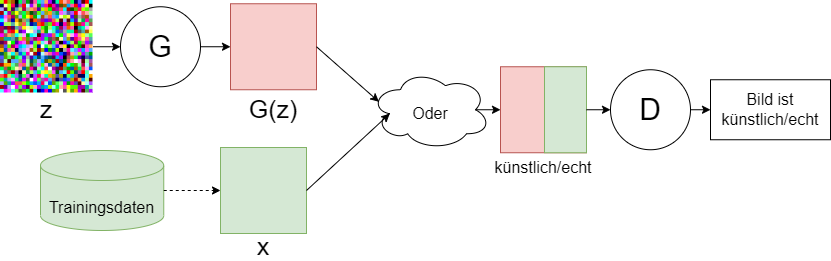
\includegraphics[width=0.8\textwidth]{../images/GANs/GAN.drawio.png}
	\caption{Zusammenspiel zwischen Generator und Diskriminator}
	\label{fig:gan}
\end{figure}
Der Eingangvektor heißt $z$. Daraus erzeugt Generator $G$ ein Bild $G(z)$. Der Diskriminator $D$ erhält entweder ein Bild $x$ aus den Trainingsdaten oder ein Bild $G(z)$ vom Generator. Darauf basierend trifft der Diskriminator entweder eine Vorhersage $D(x)$ oder $D(G(z))$, wie wahrscheinlich es ist, dass das Bild real ist. Bei der Vorhersage handelt es sich um eine Wahrscheinlichkeit zwischen $0$ und $1$. Ein Wert von $0.8$ bedeutet demnach zum Beispiel: Der Diskriminator ist sich zu 80\% sicher, dass das Bild real ist. \cite{GANs}

\paragraph{Training}
Hieraus ergibt sich die Kostenfunktion für \acp{GAN}. Sie nennt sich $V(D,G)$: \cite{Goodfellow-GANs}
\begin{equation}
   \label{eq:adv_loss}
	\min_{G} \max_{D} V(D,G) = \mathbb{E}_{x}[\log(D(x))] + \mathbb{E}_{z}[\log(1-D(G(z)))]
\end{equation}
Bei dem Training handelt es sich um ein Min-Max-Problem. Der Generator versucht die Funktion $V(G,D)$ zu minimieren, wohingegen der Diskriminator sie zu maximieren versucht. Das Ziel des Trainings ist damit nicht wie klassischerweise bei \acp{KNN}, dass die Funktion einen Wert von $0$ anstrebt. Stattdessen soll sie im Verlauf des Trainings gegen einen Wert größer als $0$ konvergieren. Hier können sich der Generator und der Diskriminator nicht weiter verbessern. Sie haben idealerweise optimale Parameter. Es wird davon gesprochen, dass $G$ und $D$ sich in einem \emph{Nash-Gleichgewicht} befinden. Dieser Begriff stammt aus der Spieltheorie und kann deshalb verwendet werden, weil ein \ac{GAN} als ein Spiel zwischen Generator und Diskriminator beschrieben werden kann. \cite{GANs}

Die Funktion $V(D,G)$ basiert auf einer logarithmischen Verlustfunktion. Der Term \ref{eq:real_adv_loss} aus der Kostenfunktion stellt die Fehlerrate des Diskriminators auf den echten Trainingsdaten dar. Die Fragestellung lautet: \emph{Wenn ich ein zufälliges Bild $x$ aus den Trainingsdaten ziehe, wie wahrscheinlich ist es, dass der Diskriminator es als echt klassifiziert?} Der Wert für $\log(D(x))$ sollte möglichst nahe $0$ sein, da für jedes echte Trainingsbild $x$ zu erwarten ist, dass $D(x)$ einen Wert nahe $1$ ausgibt.

\begin{equation}
	\label{eq:real_adv_loss}
	\mathbb{E}_{x}[\log(D(x))]
\end{equation}

Der Term \ref{eq:fake_adv_loss} beschreibt hingegen, wie viele generierte Bilder der Diskriminator als echt klassifiziert. Hierfür werden zufällige $z$ aus der Wahrscheinlichkeitsverteilung der Eingangsvektoren entnommen. Diese Verteilung kann beliebig definiert sein. Ist der Diskriminator besser trainiert als der Generator, dann ist zu erwarten, dass $D((G(z)))$ einen Wert nahe $0$ hat. Somit ist der Logarithmus ebenfalls nahe $0$. Im umgekehrten Fall nimmt der Logarithmus einen negativen Wert an. Der Betrag des Werts erhöht sich, je mehr $D(G(z))$ gegen $1$ strebt.
\begin{equation}
   \label{eq:fake_adv_loss}
	\mathbb{E}_{z}[\log(1-D(G(z)))]
\end{equation}
Der Term \ref{eq:real_adv_loss} ist nicht vom Generator abhängig, sondern lediglich von $D$ und $x$. Hierauf hat der Generator keinen Einfluss, wodurch er alleine durch diesen Teil der Kostenfunktion nicht trainiert wird. Der Diskriminator besitzt somit zwei Terme, die ihn trainieren, während der Generator nur einen besitzt. Aus diesem Grund werden dem Diskriminator in der Regel doppelt so viele unechte Daten wie echte Trainingsdaten gezeigt. Dies soll einem ungleichen Training der beiden Komponenten des \acp{GAN} entgegenwirken. Der Optimalzustand eines \acp{GAN} ist, dass der Diskriminator so gut wie möglich identifizieren kann, ob ein gegebenes Bild aus $p(x)$ stammt, während der Generator dennoch in der Lage ist, den Diskriminator zu überlisten. Das Training von \acp{GAN} gilt als empfindlich gegenüber den gewählten Hyperparametern und der Netzwerkarchitektur. \acp{GAN} wird nachgesagt, dass kleine Änderungen in den beiden genannten Aspekten die Qualität der Generierten Bildern signifikant beeinflussen können. \cite{visualApproach}

Im praktischen Einsatz wird nur der Generator des \acp{GAN} verwendet. Der Diskriminator wird ausschließlich dazu eingesetzt, mit $p(G(z))$ möglichst gut $p(x)$ zu approximieren, sodass die generierten Bilder im Optimalfall nicht von echten Trainingsdaten zu unterscheiden sind. \cite{visualApproach}
%Analog zu Kapitel \ref{chap:NoGANs}, ist die Aufgabe des Generators, Daten aus der Wahrscheinlichkeitsverteilung $p(x)$ der Trainingsdaten zu erzeugen. Der Eingangsvektor $z$ des Generators folgt einer Verteilung $p_z(z)$. Der Generator kann durch folgende Funktion beschrieben werden:

%\begin{equation}
%	G(z, \theta_{g})
%\end{equation}

%Der Generator erzeugt neue Bilder, während der Discriminator für jedes erzeugte Bild rät, ob es aus dem Trainingssatz stammt, oder ob es künstlich generiert ist. Nur der Discriminator hat dabei Zugriff auf den Trainingsdatensatz. Ihm werden klassischerweise abwechselnd Bilder aus dem Trainingssatz und erzeugte Bilder des Generators gezeigt. Die beiden Komponenten des \acp{GAN} agieren dabei stets gegeinander. Der Generator versucht den Discriminator in die Irre zu führen, dass seine generierten Bilder in Wahrheit aus dem Trainingssatz stammen würden, während der Discriminator versucht, möglichst gut zu erkennen, ob ein Bild echt ist oder nicht. Bei beiden Komponenten handelt es sich dabei um künstliche neuronale Netze \acused{KNN}(\acp{KNN}). \cite{visualApproach}

%\subsection{Spieltheorie}
%Aus spieltheoreticher Sicht kann das Gegenspiel von Generator und Discriminator auch als \emph{Nullsummenspiel} %betrachtet werden.
%Zu Beginn werden sowohl der Generator als auch der Discriminator mit zufälligen Parametern initialisiert. Dadurch ist zu erwarten, dass 


%Der Generator erzeugt Bilder, die denen des Trainingssatzes nicht änhlich sind, während der Discriminator noch nicht weiß, was die Bilder des Trainingssatzes einzigartig macht. Durch das Training verbessern sich beide Komponenten in ihren Aufgaben. Sie trainieren sich gegenseitig, da sie beide versuchen, das Spiel zu gewinnen.

%Das finale Optimum ist, dass der Discriminator so gut in der Unterscheidung zwischen echten und künstlichen Daten wird, wie mit den vorhandenen Daten nur möglich, während der Generator trotzdem in der Lage sein soll, den Discriminator zu überlisten. \cite[S. 656]{visualApproach}

%Während die Bildklassifizierung ein Minimierungsproblem ist, stellt die Bildgenerierung mittels \acp{GAN} ein Min-Max-Problem dar. Bei ersterem wird versucht, die Loss-Function zu minimieren, sodass die Predictions möglichst gut den Labels der Daten entsprechen. Bei \acp{GAN} besteht der Unterschied darin, dass einerseits der Generator die Loss-Function zu minimieren versucht, während andererseits der Discriminator sie zu maximieren versucht.

%\begin{equation}
%	\min_{G} \max_{D} V(D,G) = \mathbb{E}_{x}[\log(D(x))] + \mathbb{E}_{z}[\log(1-D(G(z)))]
%\end{equation}
Die bisher beschriebene Architektur von \acp{GAN} wird auch als \emph{Vanilla \ac{GAN}} bezeichnet. Forscher und Anwender haben seit dieser Veröffentlichung verschiedene Limitationen und Probleme bei Vanilla \acp{GAN} feststellen können. Insbesondere im Hinblick auf spezielle Einsatzgebiete. Ein hier häufig anzutreffender Begriff ist \emph{Modal Collaps}. Damit ist die Situation gemeint, dass der Generator bei beliebigem Input stets dasselbe Bild generiert. Er lernt, dass ein bestimmtes Bild den Diskriminator überlisten kann und generiert es deshalb jedes Mal, egal welchen Input man ihm zuführt. In dem Anwendungsfall dieser Arbeit könnte das zum Beispiel dazu führen, dass der Generator nur eine einzelne Art von Straßenschild generiert. Lösen lässt sich das Problem des \emph{Modal Collaps} beispielsweise mit sogenannten \acp{CycleGAN}. \cite{visualApproach}

\paragraph{CycleGANs}
\acp{CycleGAN} eignen sich für eine bestimmte Art der generativen Modellierung: Der Bild-zu-Bild Übersetzung. Hierbei soll das Modell nicht ein völlig neues Bild generieren, sondern ein vorhandenes Bild in eine andere Domäne übersetzen. Ein Beispiel dafür ist das Umwandeln von Zeichnungen in fotorealistische Bilder oder das Einfärben von schwarz-weiß Bildern. Ein entscheidender Unterschied ist somit, dass der Generator keinen zufälligen Vektor $z$ als Eingang enthält, sondern ein Bild, dass Modell in eine andere Domäne übersetzen soll. Bei solchen Anwendungsfällen sollen \acp{CycleGAN} einen Modal Collaps verhindern. Das Ziel ist, dass das erzeugte Bild des Modells immer abhängig von dem Eingangbild ist. \cite{cycleGAN}

Ein \ac{CycleGAN} besteht aus zwei miteinander gekoppelten \acp{GAN}. Generator $G$ übersetzt ein Bild $x$ in ein Bild $y$. Aus diesem $y$ soll dann Generator $F$ den Eingang $x$ rekonstruieren. Somit soll das gesamte Netzwerk nicht nur neue Bilder generieren können, sondern soll auch von einem generierten Bild zurück auf den zugeführten Eingang schließen können. Die Bilder $x$ und $y$ entstammen den Domänen $X$ und $Y$. Dabei steht $X$ zum Beispiel für Zeichnungen und $Y$ für fotorealistische Bilder. Dies lässt sich mathematisch so darstellen, dass $G$ und $F$ folgende Abbildungen implementieren: \cite{cycleGAN}

\begin{equation}
	\mathbf{G}: X\mapsto Y \: \wedge \: \mathbf{F}: Y\mapsto \hat{X}
\end{equation}

Das Modell $G$ erzeugt somit aus einem gegebenen $x$ ein $y$, wohingegen $F$ aus dem $y$ auf das $x$ schließen soll. Die Behebung des Modal Collaps findet dadurch statt, dass das Netzwerk den Output $\hat{x}$ von $F$ überprüft und diesen mit dem tatsächlichen Eingang $x$ vergleicht. Es wird überprüft, wie ähnlich sich $\hat{x}$ und $x$ sind. Liegt eine zu hohe Diskrepanz vor, kann das Netzwerk darauf schließen, dass $G$ Ausgaben erzeugt, die nicht in direkter Abhängigkeit zu $x$ stehen. \cite{cycleGAN}

Das Training von \acp{CycleGAN} basiert auf mehreren Kostenfunktionen. Die \acp{GAN} $G$ und $F$ besitzen jeweils eigene Diskriminatoren $D_y$ und $D_x$. Dadurch haben beide \acp{GAN} einen eigenen \emph{Adversarial Loss}. Damit ist die in Gleichung \ref{eq:adv_loss} beschriebene Kostenfunktion eines Vanilla \acp{GAN} gemeint. Es sei erwähnt, dass die \ac{CycleGAN}-Veröffentlichung hier von Verlustfunktionen \emph{engl: losses} mit dem Formelzeichen $\mathcal{L}$ spricht, während hier der Begriff Kostenfunktion genutzt wird. Die Formeln sind jedoch identisch, da sich die Verlustfunktionen bereits auf mehrere Trainingsbeispiele beziehen. \cite{cycleGAN}

Im Kontext von \acp{CycleGAN} ist der beschriebene Adversarial Loss für das \ac{GAN} G wie folgt definiert: \cite{cycleGAN}

\begin{equation}
	\mathcal{L}_{GAN}(G, D_Y, X, Y) = \mathbb{E}_y[\log{D_Y(y)}] + \mathbb{E}_x[\log(1-D_Y(G(x)))]
\end{equation}
Die Funktion für \ac{GAN} F ist identisch, mit dem Unterschied, dass sie von $F$ und $D_X$ statt von $G$ und $D_Y$ abhängt. Ein Unterschied zu den Vanilla \acp{GAN} ist hierbei: Bei Vanilla \acp{GAN} steht der Buchstabe $x$ für die Trainingsdaten aus der Zieldomäne. Hier sind jedoch einzelne $x$ die Eingabewerte für das \ac{CycleGAN}. Was vorher $z$ war, ist demnach hier $x$. Die Trainingsdaten aus der Zieldömäne werden mit dem Formelzeichen $y$ abgekürzt. \cite{cycleGAN}

Als weitere Kostenfunktion besitzen \acp{CycleGAN} einen \emph{Cycle Consistency Loss} (Gleichung \ref{eq:cycle-loss}). Die beiden Summanten der Gleichung setzen sich daraus zusammen, wie weit die Pixelwerte von den generierten Bildern und den echten Bildern auseinander liegen. Mit $G(x)$ wird ein Bild $\hat{y}$ generiert, $F$ generiert anschließend aus diesem $\hat{y}$ wieder ein $\hat{x}$. Wenn $\hat{x}$ und $x$ möglichst ähnlich sind, dann kann davon ausgegangen werden, dass die generierten Bilder des Netzwerks $G$ in direkter Abhängigkeit von dem Input $X$ stehen. Was hierbei berechnet wird, ist die durschnittliche, absolute Abweichung der Pixelwerte. \cite{cycleGAN}
\begin{equation}
   \label{eq:cycle-loss}
	\mathcal{L}_{cyc}(G, F) = \mathbb{E}_x[\mathcal{L}_{1}(F(G(x))-x)] + \mathbb{E}_y[\mathcal{L}_{1}(G(F(y))-y)]
\end{equation}
Um die gesamten Kosten des \acp{CycleGAN} zu erhalten, werden die bisher beschriebenen Kostenfunktionen addiert. Der Cycle Consistency Loss $L_{cyc}(G, F)$ wird dabei mit einem absoluten Wert $\lambda$ multipliziert, um die Kosten dieser Funktion im Vergleich zu den \emph{Adversarial Losses} gewichten zu können. In der Veröffentlichung der \acp{CycleGAN} wird ein $\lambda$ von $10$ verwendet. Somit wird mit einem vergleichweise hohen Gewicht versehen, dass die generierten Bilder in direkter Abhängigkeit zu den Eingangswerten des \acp{CycleGAN} stehen. Der Wert $\lambda$ stellt einen Hyperparamer dar. \cite{cycleGAN}
\begin{equation}
	\mathcal{L}(G, F, D_X, D_Y) = \mathcal{L}_{GAN}(G, D_Y, X, Y) + \mathcal{L}_{GAN}(F, D_X, Y, X) + \lambda \cdot \mathcal{L}_{cyc}(G, F)
\end{equation}
\cite{cycleGAN}

Einige Implementierungen teilen die Kostenfunktion auf einzelne Verluste für jeweils die Generatoren $G$ und $F$ sowie die Diskriminatoren $D_y$ und $D_x$ auf: \cite{cyclegan-tutorial} \cite{cyclegan-resnet}
\begin{subequations}
   \label{eq:cyclegan-losses}
   \begin{align}
      \mathcal{L}_G = \mathbb{E}_x [\log(D_Y(G(x)))] + \mathcal{L}_{cyc}(G, F) \\ 
      \mathcal{L}_F = \mathbb{E}_y [\log(D_X(F(y)))] + \mathcal{L}_{cyc}(G, F) \\
      \mathcal{L}_{D_y} = 0.5 \cdot \mathcal{L}_{GAN}(G, D_Y, X, Y) \\
      \mathcal{L}_{D_x} = 0.5 \cdot \mathcal{L}_{GAN}(F, D_X, Y, X)
\end{align}
\end{subequations}
Das erlaubt ein separates Training der einzelnen \acp{KNN} des \acp{CycleGAN}. Die Generatoren besitzen in ihrer Kostenfunktion lediglich den Teil des Adversarial Loss, den sie beeinflussen können. Dieser ist jedoch so abgeändert, dass die Generatoren einen möglichst hohen Wert für $D_y(G(x))$ beziehungsweise $D_x(F(y))$ anstreben. In diesem Fall führt dort ein Wert nahe $1$ zu Kosten von Nahe $0$. Das entspricht dem, dass die Generatoren versuchen, den entsprechenden Diskriminator zu Falschaussagen zu verleiten.
 
Die Qualität der Diskriminatoren wird anhand des gesamten Adversarial Loss gemessen. Diese Kosten werden bei den Diskriminatoren mit $0.5$ multipliziert, damit die Diskriminatoren nicht schneller trainiert werden als die Generatoren \cite{cyclegan-tutorial}. Stattdessen wäre es auch möglich, die Trainingschritte der Generatoren doppelt so oft durchzuführen, wie die der Diskriminatoren \cite{visualApproach}.

Die Basis für $G$ und $F$ ist eine bestimmte \ac{CNN}-Architektur, die sich \ac{ResNet} nennt. Diese haben Forscher von Microsoft Research im Jahre 2015 eingeführt. Die Autoren der \ac{CycleGAN} Veröffentlichung wählen diese Architektur, weil sie in einem ähnlichen Anwendungsfall bei anderen Autoren überzeugende Resultate gezeigt habe. Der Grundbaustein eines \ac{ResNet}, der sogenannte \emph{Residual Block},fdass  ist in Abbildung \ref{fig:residual-block} dargestellt. \cite{resnet} \Cite{cycleGAN}

\begin{figure}[h]
   \centering
   \includegraphics[width=0.4\textwidth]{images/residual block.png}
   \caption{Residual Block eines ResNet \cite{resnet}}
   \label{fig:residual-block}
\end{figure}

Residual Blocks besitzen zwei Pfade. Ein Pfad enthält mindestens einen Convolutional Layer, der den Eingangswert $x$ verändert. Das Ergebnis dieser Berechnung ist ein neuer Wert $\mathcal{F}(x)$. Der andere Pfad gibt den Eingangswert unverändert weiter und addiert ihn auf den Wert $\mathcal{F}(x)$. Das Ergebnis der beiden Pfade ist ein neuer Wert $\mathcal{F}(x) + x$. Die Aktivierungsfunktion des Residual Block erhält diese Summe als Eingabe. Residual Blocks beschleunigen laut den Autoren das Training von tiefen neuronalen Netzen und erlauben damit Netzwerkarchitekturen mit mehr Schichten als klassische \ac{CNN}. \cite{resnet}

\paragraph{Conditional GANs}
Eine weitere Möglichkeit, die Generierung von \acp{GAN} zu steuern, sind sogenannte \acp{cGAN}. Dabei erhält der Generator zusätzlich zu dem zufällig erzeugten Eingangsvektor $z$ noch eine Bedingung $x$. Das kann es zum Beispiel eine Zahl sein, die für ein bestimmtes Objekt steht, welches das \acp{cGAN} erzeugen soll. Außerdem kann es sich beispielsweise um natürliche Sprache handeln, die Objekt beschreibt, das der Generator erzeugen soll. Der Diskriminator überprüft dann nicht nur, ob das Bild echt oder künstlich ist, sondern auch, ob es der Bedingung $x$ entspricht.

Die Kostenfunktion lautet dann wie folgt: \cite{pix2pix}
\begin{equation}
   \label{eq:cond_gan}
   \min_{G} \max_{D} V(D,G) = \mathbb{E}_{x, y}[\log(D(x, y))] + \mathbb{E}_{x,z}[\log(1-D(x, (G(x, z))))]
\end{equation}
Wobei: \newline
\emph{\null\quad\quad $x$: Bedingung, die der Generator enthält beziehungsweise zu dem Bild $y$ gehört \newline
\null\quad\quad $y$: Reales Bild aus den Trainingsdaten}

Bei der Generierung von Straßenschildern könnte das $x$ zum Beispiel eine Zahl sein, die für das Straßenschild steht, das der Generator erzeugen soll.

Zusätzlich ist es möglich, solche \acp{cGAN} zur Bild-zu-Bild Übersetzung zu verwenden. Darauf bezieht sich gezielt eine bestimmte Veröffentlichung \cite{pix2pix}. Dabei sorgt der Vektor $z$ dafür, dass die Ausgabe des Generators nicht-deterministisch ist. Die Autoren der Veröffentlichung schreiben jedoch, dass der Generator das $z$ meistens weitgehend ignoriert und dadurch wenig Varianz in den generierten Bildern zeigt. Der Quellcode der Veröffentlichung trägt den Namen \emph{pix2pix}. \cite{pix2pix}

Innerhalb von \emph{pix2pix} basiert der Generator auf einem \emph{U-Net}. Dies ist eine Architektur aus dem Jahre 2015, die das Eingangsbild zunächst auf eine geringere Anzahl an Parametern Kodiert und anschließend zu einem neuen Bild dekodiert. Die Architektur ähnelt somit konzeptionell der eines Autoencoders. U-Nets sind ursprünglich für die Segmentierung, also das markieren von bestimmten Bereichen in Bildern, für mezidizinische Zwecke entwickelt worden. Die Architektur dieser Modelle stellt Abbildung \ref{fig:unet} dar. \cite{unet} \cite{pix2pix}

\begin{figure}[h]
   \centering
   \includegraphics[width=0.7\linewidth]{images/unet.png}
   \caption{Architektur eines U-Net \cite{unet}}
   \label{fig:unet}
\end{figure}

Ihren Namen erhalten U-Nets durch die u-förmige Architektur. Sie erhalten ein Bild, extrahieren mittels mehrer Convolutional Layer daraus Merkmale und geben diese dann an weitere Convolutional Layer weiter, die hieraus ein neues Bild erzeugen. U-Nets besitzen in jeder kodierenden Schicht Direktverbindungen zu der zugehörigen dekodierenden Schicht. Das ist in der Abbildung durch graue Pfeile dargestellt. Ein Vorteil dieser Verbindungen ist, dass dadurch weniger Informationen zwischen der Kodierung und der Dekodierung verloren gehen. \cite{unet}

Der Diskriminator des pix2pix \ac{cGAN} verwendet eine Architektur, die sich \emph{PatchGAN} nennt. Die Besonderheit ist hierbei, dass der Diskriminator nicht einzelne Pixel betrachtet, sondern Teile eines Bilds als echt oder unecht klassifizieren kann. Die gleiche Diskriminatorarchitektur verwendet auch die Veröffentlichung der \acp{CycleGAN}. \cite{pix2pix} \cite{cycleGAN}

Einer der Hauptunterschiede zwischen pix2pix und \acp{CycleGAN} ist, dass pix2pix gepaarte Trainingsdaten benötigt. Zu jedem $x$ müssen die Trainingsdaten das erwartete $y$ enthalten. Nur so kann der Diskriminator lernen, welche Bilder zu einer bestimmten Bedingung gehören. \acp{CycleGAN} brauchen das nicht. Sie benötigen Trainingsbilder aus der Domäne $X$ und aus der Domäne $Y$, diese müssen jedoch in keiner Beziehung zueinander stehen. Deshalb fallen \acp{cGAN} unter das überwachte Lernen, während \acp{CycleGAN} dem unüberwachten Lernen zuzuordnen sind. \cite{pix2pix} \cite{cycleGAN}

Analog zu den Vanilla \acp{GAN} berechnen \acp{CycleGAN} und \acp{cGAN} keine direkte Wahrscheinlichkeitsverteilung der Trainingsdaten. Das Spiel zwischen Generator und Diskriminator sorgt implizit für eine Abbildung zwischen $\hat{p}(x)$ und $p(x)$. In der in Abbildung \ref{fig:generativeModelsTaxonomy} gezeigten Taxonomie befinden sie sich aus diesem Grund in der Kategorie \emph{Implizite Wahrscheinlichkeitsdichte}. \cite{pix2pix} \cite{cycleGAN}

%In dieser Studienarbeit sollen \acp{GAN} zur Generierung künstlicher Bilder von Straßenschildern eingesetzt %werden. Dies ist jedoch nicht die einzige Möglichkeit, wie mittels \acp{KNN} künstliche Bilder erzeugt werden %können. In diesem Kapitel werden daher weitere Methoden vorgestellt, die ebenfalls dazu eingesetzt werden können.

%Eines der bisher genannten Beispiele für \acp{KNN} ist die Umsetzung eines Katzenklassifikators. Diese sogenannten %diskriminativen Modelle setzen grundlegend folgende Wahrscheinlichkeitsfunktion um:
%\begin{equation}
%   p(y|x)
%\end{equation}
%Bei einem Eingang $x$ soll das Modell die Wahscheinlichkeit für jeden Ausgang $y$ bestimmen. Zeigt man einem %Katzenklassifikator ein Bild auf dem keine Katze zu sehen ist, so soll $p(\mathrm{Katze}|x)$ gering sein. Die %Wahrscheinlichkeiten einer Wahrscheinlichkeitsverteilung müssen zusammen den Wert \emph{eins} ergeben, wodurch im %Umkehrschluss der Ausgang $p(\mathrm{KeineKatze}|x)$ eine hohe Wahrscheinlichkeit liefert. Um diese Verteilung %erlernen zu können, ist Supervised Learning notwendig.

%Generative Netze besitzen eine andere Aufgabe. Sie sollen neue Verteilungen generieren. Diese Verteilungen sollen %möglichst ähnlich der Verteilung sein, auf die das Modell trainiert wurde. Das Modell bestimmt, wie wahrscheinlich %es ist, dass ein gegebenes $x$ aus der Verteilung stammt. Konkret bezogen auf den Kontext dieser Studienarbeit: %Gibt man dem generativen Modell ein Bild, soll es bestimmen, wie wahrscheinlich es ist, dass dies ein real %aufgenommenes Foto eines Straßenschildes ist. Es wird folgende Wahrscheinlichkeitsfunktion umgesetzt:
%\begin{equation}
%   p(x)
%\end{equation}
%Wobei $p(x)$ als die Wahrscheinlichkeit interpretiert werden kann, dass ein gegebenes $x$ aus der Verteilung der %Trainingsdaten stammt.

%\subsection{Boltzmann Maschinen}
%\subsection{Deep Belief Netzwerke}